% (C) Marc Lijour, 2016-2017
% Licensed under a Creative Commons License BY-SA
% https://creativecommons.org/licenses/by-sa/2.5/ca/
% Presentation for the Small Business Digitization Initiative (SBDI) training program
% see http://www.ictc-ctic.ca/small-business-digitization-initiative/ 
% authored by Marc Lijour, December 2016
% for the session running from January 2017 to September 2017
% 
% Variables
% TODO set the variables
% ---------------------- USER-DEFINED --------------------------------
\newcommand{\SFLtitle}{Digitization~Theory~2}
\newcommand{\SFLlongtitle}{Competing with Technology and Innovation}
\newcommand{\SFLsubtitle}{Small Business Digitization Initiative (SBDI) - Day 2}
\newcommand{\SFLauthor}{Marc~Lijour}
\newcommand{\SFLdate}{March~21, 2017}
\newcommand{\SFLsubject}{Digitization Theory}
% --------------------------------------------------------------------
% Template
% (C) Savoir-faire Linux, 2016 (this document and associated logos and art)
% This document is licensed under a Creative Commons License BY-SA (feel free to use the code, but all rights are reserved for logos and art)
% https://creativecommons.org/licenses/by-sa/2.5/ca/
% Savoir-faire Linux presentation template for LaTeX
% authored by Marc Lijour, December 2016
% This template comes with a first page on a blue background
% Possible improvement in future iterations
% - Test and fix as needed to work on xetex (to use Ubuntu fonts)
% === USAGE===
% Create a file for your LaTeX content (slides, etc), in which you must do the following:
% TODO 1 - set variables defined below
% TODO 2 - include this code by calling: % (C) Savoir-faire Linux, 2016 (this document and associated logos and art)
% This document is licensed under a Creative Commons License BY-SA (feel free to use the code, but all rights are reserved for logos and art)
% https://creativecommons.org/licenses/by-sa/2.5/ca/
% Savoir-faire Linux presentation template for LaTeX
% authored by Marc Lijour, December 2016
% This template comes with a first page on a blue background
% Possible improvement in future iterations
% - Test and fix as needed to work on xetex (to use Ubuntu fonts)
% === USAGE===
% Create a file for your LaTeX content (slides, etc), in which you must do the following:
% TODO 1 - set variables defined below
% TODO 2 - include this code by calling: % (C) Savoir-faire Linux, 2016 (this document and associated logos and art)
% This document is licensed under a Creative Commons License BY-SA (feel free to use the code, but all rights are reserved for logos and art)
% https://creativecommons.org/licenses/by-sa/2.5/ca/
% Savoir-faire Linux presentation template for LaTeX
% authored by Marc Lijour, December 2016
% This template comes with a first page on a blue background
% Possible improvement in future iterations
% - Test and fix as needed to work on xetex (to use Ubuntu fonts)
% === USAGE===
% Create a file for your LaTeX content (slides, etc), in which you must do the following:
% TODO 1 - set variables defined below
% TODO 2 - include this code by calling: \input{sfl-presentation-template-blue-EN}
% TODO 3 - Start the document as usual and you're in business; just use \begin{document} and don't forget to conclude with \end{document}
% TODO 4 - Use the custom method \SFLcoverpage instead of \titlepage to create your cover page
% Voilà!
%
\documentclass{beamer}
\usepackage{etoolbox}
% Variables
% ---------------------- USER-DEFINED --------------------------------
\ifdef{\SFLtitle}{}{\newcommand{\SFLtitle}{\color{red}Title TBD}}
\ifdef{\SFLlongtitle}{}{\newcommand{\SFLlongtitle}{\color{red}Long title TBD}}
\ifdef{\SFLsubtitle}{}{\newcommand{\SFLsubtitle}{\color{red}Subtitle TBD}}
\ifdef{\SFLauthor}{}{\newcommand{\SFLauthor}{\color{red}Author TBD}}
\ifdef{\SFLdate}{}{\newcommand{\SFLdate}{\color{red}Date TBD}}
\ifdef{\SFLsubject}{}{\newcommand{\SFLsubject}{\color{red}Subject TBD}}
% --------------------------------------------------------------------
\usetheme{Boadilla}
% Set color close to Savoir-faire Linux standard
\definecolor{beamer@blendedblue}{RGB}{86,176,201}
% Cover Page
\title[\SFLtitle] {\SFLlongtitle}
\subtitle{\SFLsubtitle}
\author{\SFLauthor}
\date{\SFLdate}
\subject{\SFLsubject}
\usepackage{tikz}
% -- possible approach through modif of the template (abandonned for now)
%\addtobeamertemplate{title page}{
%    \tikz[remember picture,overlay]
%        \node at ([xshift=0cm,yshift=0cm]current page.center) 
%		 {
\includegraphics[width=\paperwidth, height=\paperheight]{./images/sfl-background-blue}};
%}{}
%\setbeamercolor{title page}{fg=white}
%\setbeamercolor{titlelike}{fg=white}
%\setbeamertemplate{navigation symbols}{}
% Try Xetex to use system fonts (pdflatex makes it hard to import a font)
%\usepackage{fontspec}
%\setsansfont{Ubuntu}
%\setmonofont{Ubuntu Mono}
%
%\usepackage[absolute,overlay]{textpos}
%\setlength{\TPHorizModule}{\paperwidth}
%\setlength{\TPVertModule}{\paperheight}
% -- create a custom (command) title page -which has the benefit of not affecting the settings for the rest of the presentation
\newcommand{\SFLcoverpage}{\frame[plain]{
	\tikz[remember picture,overlay] {
        	\node(bkgd) at ([xshift=0cm,yshift=0cm]current page.center) 
			{
\includegraphics[width=\paperwidth, height=\paperheight]{../templates/images/sfl-background-blue}};
        	\node(logo) at ([xshift=0cm,yshift=2.5cm]current page.center) 
		 	{
\includegraphics[scale=.20]{../templates/images/logo-sfl-blanc-rgb-72dpi}};
	}
	\tikz[remember picture,overlay] {
        	\node(title) at ([xshift=0cm,yshift=1cm]current page.center) 
			{\Large\color{white}\textbf{{\SFLlongtitle}}};
        	\node(subtitle) at ([xshift=0cm,yshift=.2cm]current page.center) 
			{\small\color{white}\emph{\SFLsubtitle}};
        	\node(author) at ([xshift=0cm,yshift=-2cm]current page.center) 
			{\small\color{white}By~\SFLauthor};
        	\node(date) at ([xshift=0cm,yshift=-2.5cm]current page.center) 
			{\tiny\color{white}\SFLdate};
        	\node(footnote) at ([xshift=0cm,yshift=-4cm]current page.center) 
			{\TINY\color{white}\emph{The registered trademark Linux$^\circledR$ is used pursuant to a sublicense from LMI, the exclusive licensee of Linus Torvalds, owner of the mark on a world-wide basis.}};
    	}
}}
%
% This sets a Savoir-faire Linux logo at the bottom right corner of each page
\logo{
\includegraphics[scale=.1]{../templates/images/logo-sfl-250.png}}
\AtBeginSection[]
{
  \begin{frame}
    \frametitle{Table of Contents}
    \tableofcontents[currentsection]
  \end{frame}
}
%\usepackage[format=plain,justification=raggedright,singlelinecheck=false]{caption}
\usepackage[format=plain,justification=justified,singlelinecheck=false]{caption}
\usepackage[utf8]{inputenc}
\usepackage{dirtytalk}
\usepackage{wrapfig}
\usepackage{hyperref}
\usepackage{verbatim}
\usepackage{mathabx}
%\usepackage{MnSymbol}


% TODO 3 - Start the document as usual and you're in business; just use \begin{document} and don't forget to conclude with \end{document}
% TODO 4 - Use the custom method \SFLcoverpage instead of \titlepage to create your cover page
% Voilà!
%
\documentclass{beamer}
\usepackage{etoolbox}
% Variables
% ---------------------- USER-DEFINED --------------------------------
\ifdef{\SFLtitle}{}{\newcommand{\SFLtitle}{\color{red}Title TBD}}
\ifdef{\SFLlongtitle}{}{\newcommand{\SFLlongtitle}{\color{red}Long title TBD}}
\ifdef{\SFLsubtitle}{}{\newcommand{\SFLsubtitle}{\color{red}Subtitle TBD}}
\ifdef{\SFLauthor}{}{\newcommand{\SFLauthor}{\color{red}Author TBD}}
\ifdef{\SFLdate}{}{\newcommand{\SFLdate}{\color{red}Date TBD}}
\ifdef{\SFLsubject}{}{\newcommand{\SFLsubject}{\color{red}Subject TBD}}
% --------------------------------------------------------------------
\usetheme{Boadilla}
% Set color close to Savoir-faire Linux standard
\definecolor{beamer@blendedblue}{RGB}{86,176,201}
% Cover Page
\title[\SFLtitle] {\SFLlongtitle}
\subtitle{\SFLsubtitle}
\author{\SFLauthor}
\date{\SFLdate}
\subject{\SFLsubject}
\usepackage{tikz}
% -- possible approach through modif of the template (abandonned for now)
%\addtobeamertemplate{title page}{
%    \tikz[remember picture,overlay]
%        \node at ([xshift=0cm,yshift=0cm]current page.center) 
%		 {
\includegraphics[width=\paperwidth, height=\paperheight]{./images/sfl-background-blue}};
%}{}
%\setbeamercolor{title page}{fg=white}
%\setbeamercolor{titlelike}{fg=white}
%\setbeamertemplate{navigation symbols}{}
% Try Xetex to use system fonts (pdflatex makes it hard to import a font)
%\usepackage{fontspec}
%\setsansfont{Ubuntu}
%\setmonofont{Ubuntu Mono}
%
%\usepackage[absolute,overlay]{textpos}
%\setlength{\TPHorizModule}{\paperwidth}
%\setlength{\TPVertModule}{\paperheight}
% -- create a custom (command) title page -which has the benefit of not affecting the settings for the rest of the presentation
\newcommand{\SFLcoverpage}{\frame[plain]{
	\tikz[remember picture,overlay] {
        	\node(bkgd) at ([xshift=0cm,yshift=0cm]current page.center) 
			{
\includegraphics[width=\paperwidth, height=\paperheight]{../templates/images/sfl-background-blue}};
        	\node(logo) at ([xshift=0cm,yshift=2.5cm]current page.center) 
		 	{
\includegraphics[scale=.20]{../templates/images/logo-sfl-blanc-rgb-72dpi}};
	}
	\tikz[remember picture,overlay] {
        	\node(title) at ([xshift=0cm,yshift=1cm]current page.center) 
			{\Large\color{white}\textbf{{\SFLlongtitle}}};
        	\node(subtitle) at ([xshift=0cm,yshift=.2cm]current page.center) 
			{\small\color{white}\emph{\SFLsubtitle}};
        	\node(author) at ([xshift=0cm,yshift=-2cm]current page.center) 
			{\small\color{white}By~\SFLauthor};
        	\node(date) at ([xshift=0cm,yshift=-2.5cm]current page.center) 
			{\tiny\color{white}\SFLdate};
        	\node(footnote) at ([xshift=0cm,yshift=-4cm]current page.center) 
			{\TINY\color{white}\emph{The registered trademark Linux$^\circledR$ is used pursuant to a sublicense from LMI, the exclusive licensee of Linus Torvalds, owner of the mark on a world-wide basis.}};
    	}
}}
%
% This sets a Savoir-faire Linux logo at the bottom right corner of each page
\logo{
\includegraphics[scale=.1]{../templates/images/logo-sfl-250.png}}
\AtBeginSection[]
{
  \begin{frame}
    \frametitle{Table of Contents}
    \tableofcontents[currentsection]
  \end{frame}
}
%\usepackage[format=plain,justification=raggedright,singlelinecheck=false]{caption}
\usepackage[format=plain,justification=justified,singlelinecheck=false]{caption}
\usepackage[utf8]{inputenc}
\usepackage{dirtytalk}
\usepackage{wrapfig}
\usepackage{hyperref}
\usepackage{verbatim}
\usepackage{mathabx}
%\usepackage{MnSymbol}


% TODO 3 - Start the document as usual and you're in business; just use \begin{document} and don't forget to conclude with \end{document}
% TODO 4 - Use the custom method \SFLcoverpage instead of \titlepage to create your cover page
% Voilà!
%
\documentclass{beamer}
\usepackage{etoolbox}
% Variables
% ---------------------- USER-DEFINED --------------------------------
\ifdef{\SFLtitle}{}{\newcommand{\SFLtitle}{\color{red}Title TBD}}
\ifdef{\SFLlongtitle}{}{\newcommand{\SFLlongtitle}{\color{red}Long title TBD}}
\ifdef{\SFLsubtitle}{}{\newcommand{\SFLsubtitle}{\color{red}Subtitle TBD}}
\ifdef{\SFLauthor}{}{\newcommand{\SFLauthor}{\color{red}Author TBD}}
\ifdef{\SFLdate}{}{\newcommand{\SFLdate}{\color{red}Date TBD}}
\ifdef{\SFLsubject}{}{\newcommand{\SFLsubject}{\color{red}Subject TBD}}
% --------------------------------------------------------------------
\usetheme{Boadilla}
% Set color close to Savoir-faire Linux standard
\definecolor{beamer@blendedblue}{RGB}{86,176,201}
% Cover Page
\title[\SFLtitle] {\SFLlongtitle}
\subtitle{\SFLsubtitle}
\author{\SFLauthor}
\date{\SFLdate}
\subject{\SFLsubject}
\usepackage{tikz}
% -- possible approach through modif of the template (abandonned for now)
%\addtobeamertemplate{title page}{
%    \tikz[remember picture,overlay]
%        \node at ([xshift=0cm,yshift=0cm]current page.center) 
%		 {
\includegraphics[width=\paperwidth, height=\paperheight]{./images/sfl-background-blue}};
%}{}
%\setbeamercolor{title page}{fg=white}
%\setbeamercolor{titlelike}{fg=white}
%\setbeamertemplate{navigation symbols}{}
% Try Xetex to use system fonts (pdflatex makes it hard to import a font)
%\usepackage{fontspec}
%\setsansfont{Ubuntu}
%\setmonofont{Ubuntu Mono}
%
%\usepackage[absolute,overlay]{textpos}
%\setlength{\TPHorizModule}{\paperwidth}
%\setlength{\TPVertModule}{\paperheight}
% -- create a custom (command) title page -which has the benefit of not affecting the settings for the rest of the presentation
\newcommand{\SFLcoverpage}{\frame[plain]{
	\tikz[remember picture,overlay] {
        	\node(bkgd) at ([xshift=0cm,yshift=0cm]current page.center) 
			{
\includegraphics[width=\paperwidth, height=\paperheight]{../templates/images/sfl-background-blue}};
        	\node(logo) at ([xshift=0cm,yshift=2.5cm]current page.center) 
		 	{
\includegraphics[scale=.20]{../templates/images/logo-sfl-blanc-rgb-72dpi}};
        	\node(CC-BY-SA) at ([xshift=5cm,yshift=-3.5cm]current page.center) 
			{\href{https://creativecommons.org/licenses/by-sa/2.5/ca/}{
\includegraphics[scale=.4]{../templates/images/CC-BY-SA-403x141}}};
	}
	\tikz[remember picture,overlay] {
        	\node(title) at ([xshift=0cm,yshift=1cm]current page.center) 
			{\Large\color{white}\textbf{{\SFLlongtitle}}};
        	\node(subtitle) at ([xshift=0cm,yshift=.2cm]current page.center) 
			{\small\color{white}\emph{\SFLsubtitle}};
        	\node(author) at ([xshift=0cm,yshift=-2cm]current page.center) 
			{\small\color{white}By~\SFLauthor};
        	\node(date) at ([xshift=0cm,yshift=-2.5cm]current page.center) 
			{\tiny\color{white}\SFLdate};
        	\node(footnote) at ([xshift=0cm,yshift=-4cm]current page.center) 
			{\TINY\color{white}\emph{The registered trademark Linux$^\circledR$ is used pursuant to a sublicense from LMI, the exclusive licensee of Linus Torvalds, owner of the mark on a world-wide basis.}};
    	}
}}
%
% This sets a Savoir-faire Linux logo at the bottom right corner of each page
\logo{
	
\includegraphics[scale=.1]{../templates/images/logo-sfl-250.png}
}
\AtBeginSection[]
{
  \begin{frame}
    \frametitle{Table of Contents}
    \tableofcontents[currentsection]
  \end{frame}
}
%\usepackage[format=plain,justification=raggedright,singlelinecheck=false]{caption}
\usepackage[format=plain,justification=justified,singlelinecheck=false]{caption}
\usepackage[utf8]{inputenc}
\usepackage{dirtytalk}
\usepackage{wrapfig}
\usepackage{hyperref}
\usepackage{verbatim}
\usepackage{mathabx}
%\usepackage{MnSymbol}


% Extra packages
\usepackage{amssymb}
\usepackage{amsmath}
\usepackage[american]{babel}
\usepackage{csquotes}
\usepackage[backend=biber,style=apa]{biblatex}
\DeclareLanguageMapping{american}{american-apa}
% Use one bib file per section
\addbibresource{references-strategy-intro.bib}
\addbibresource{references-global-competition.bib}
\definecolor{links}{HTML}{2A1B81}
\hypersetup{colorlinks,linkcolor=,urlcolor=links}
\usepackage{booktabs}
\setlength{\heavyrulewidth}{1.5pt}
\setlength{\abovetopsep}{4pt}
\usepackage{array}
\newcolumntype{L}[1]{>{\raggedright\let\newline\\\arraybackslash\hspace{0pt}}m{#1}}
\newcolumntype{C}[1]{>{\centering\let\newline\\\arraybackslash\hspace{0pt}}m{#1}}
\newcolumntype{R}[1]{>{\raggedleft\let\newline\\\arraybackslash\hspace{0pt}}m{#1}}
% Start of the document
\begin{document}
% Cover page
% Do not use this: \frame{\titlepage}
% use this instead:
\SFLcoverpage

% Morning: Introduction to Strategy (definitions, external view, internal view) 
% (C) Marc Lijour, 2016-2017 
% Licensed under a Creative Commons License BY-SA
% https://creativecommons.org/licenses/by-sa/2.5/ca/
% Presentation for the Small Business Digitization Initiative (SBDI) training program
% see http://www.ictc-ctic.ca/small-business-digitization-initiative/ 
% authored by Marc Lijour, December 2016
% for the session running from January 2017 to September 2017
% 
% ======================================================================================================
%                                      STRATEGY - INTRODUCTION
% ======================================================================================================
\section{Introduction to Business Strategy}
% --------------------- Definition --------------------------
\subsection{What is Strategy?}
\frame{
	\frametitle{Introduction to Business Strategy}
	\framesubtitle{The origins of Strategy}
	\begin{itemize}
		\item ``The Art of War'' from Sun Tzu (5-4$^{th}$ century BC)
		\pause
		\item Greek stratēgia (Office of General)
		\pause
		\item Business Strategy becomes popular after WWII and with the creation of Business Schools
	\end{itemize}
}

\frame{
	\frametitle{Introduction to Business Strategy}
	\framesubtitle{The meaning of Strategy}
	\begin{alertblock}{Political Campaign Strategy}
		Pick a candidate from the recent USA Presidential Election, and comment on his/her strategy.
	\end{alertblock}
}

\frame{
	\frametitle{Introduction to Business Strategy}
	\framesubtitle{Different ways to think about Strategy (\cite{mintzberg2005strategy})}
	\begin{figure}
	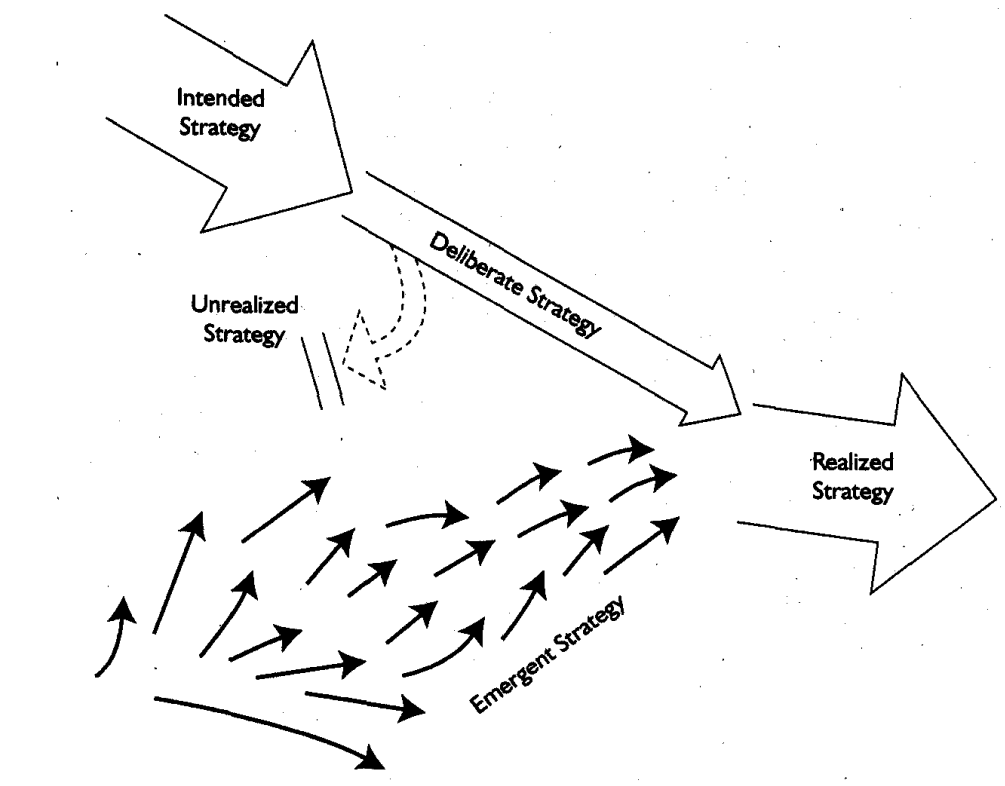
\includegraphics[height=7cm]{../pics/mintzberg-strategies-deliberate-and-emergent}
	\end{figure}
}

\frame{
	\frametitle{Introduction to Business Strategy}
	\framesubtitle{The 5 Ps of Strategy (\cite{mintzberg2005strategy})}
	\begin{itemize}
		\item Strategy as a Plan (\emph{looking ahead to the future})
		\pause
		\item Strategy as a Pattern (\emph{looking at where we've been going})
		\pause
		\item Strategy as a Position (\emph{placing products on specific markets})
		\pause
		\item Strategy as a Perspective (\emph{a somewhat personal way of doing things})
		\pause
		\item Strategy as a Ploy (\emph{acting as a mean to an end})
	\end{itemize}
}

\frame{
	\frametitle{Introduction to Business Strategy}
	\framesubtitle{Technology, Innovation, and Strategy}
	\begin{block}{Opportunity}
		Technological Innovation creates new opportunities for strategic players.
	\end{block}
}

\frame{
	\frametitle{Introduction to Business Strategy}
	\framesubtitle{Business Goals}
	\begin{alertblock}{Discussion}
		What is the main purpose of a business?
	\end{alertblock}
}

\frame{
	\frametitle{Introduction to Business Strategy}
	\framesubtitle{Two ways to create Value}
	\begin{enumerate}
		\item Production
		\item Commerce (\emph{arbitrage})
	\end{enumerate}
}

\frame{
	\frametitle{Introduction to Business Strategy}
	\framesubtitle{Most Profitable Industries --by Net Profit Margin (\cite{inc2016})}
	\begin{enumerate}
		\item Accounting, tax prep, bookkeeping, payroll services: 18.3\%
		\item Legal services: 17.4\%
		\item Lessors of real estate: 17.4\%
		\item Outpatient care centers: 15.9\%
		\item Offices of real estate agents and brokers: 14.8\%
		\item Offices of other health practitioners: 14.2\%
		\item Offices of dentists: 14.1\%
		\item Specialized design services: 12.8\%
		\item Automotive equipment rental and leasing: 12.5\%
		\item Activities related to real estate: 12.3\%
	\end{enumerate}
}

\frame{
	\frametitle{Introduction to Business Strategy}
	\framesubtitle{Estimating Profit}
	\begin{alertblock}{Discussion}
		Should we start an accounting business?	% lead toward investment valuation and cost of capital
	\end{alertblock}
}

\frame{
	\frametitle{Introduction to Business Strategy}
	\framesubtitle{Estimating Profit}
	\begin{enumerate}
		\item Accounting Profit = Total Revenue - Total Cost
		\item Net Profit Margin = Accounting Profit / Total Revenue 
		\item Economic Value Added (EVA)\newline{}= Accounting Profit - Cost of Capital - Taxes
	\end{enumerate}
}

\frame{
	\frametitle{Introduction to Business Strategy}
	\framesubtitle{Estimating Enterprise Value}
	\begin{equation}
		V = \sum_{t}\frac{C_t}{(1+r)^t}
	\end{equation}
	\begin{itemize}
		\item V: Value of the Business
		\item $C_t$: Cash Flow at year t
		\item r: discount rate i.e. weighted average cost of capital (WACC)
	\end{itemize}
}

\frame{
	\frametitle{Introduction to Business Strategy}
	\framesubtitle{Various ways to assess value}
	\begin{itemize}
		\item Economic Profit (Milton Friedman: ``the one and only one social responsibility of business [is] to increase its profits'') 
		\pause
		\item Triple Bottom Line (e.g. GRI Reporting) also looks at Social and Environmental value
		\pause
		\item Companies with a good track record of providing shareholder value generally have a mission transcending pure economic profit
	\end{itemize}
}

\frame{
	\frametitle{Introduction to Business Strategy}
	\framesubtitle{Values, Vision, and Mission Statements}
	\begin{itemize}
		\item Values: what a business stands for (honesty, quality, innovation\ldots), can be ethical
		\pause
		\item Vision: what a company wishes to become
		\pause
		\item Mission: more concrete, corporate purpose in the near future
		\pause
		\item Goals: general targets
	\end{itemize}
}

\frame{
	\frametitle{Introduction to Business Strategy}
	\framesubtitle{Two ways of Achieving Profitability}
	\begin{enumerate}
		\item Operate in an attractive industry
		\item Establishing a competitive advantage over rivals (\emph{better})
	\end{enumerate}
}

% --------------------- External View --------------------------
\subsection{The External View (where to fish)}
\begin{frame}[c]{The External View}
	\centering
	\Huge{How to find the best position to generate profit?}
\end{frame}

\frame{
	\frametitle{The External View}
	\framesubtitle{Intensity of Competition}
	\begin{itemize}
		\item Minimum (near zero): Monopoly
		\item More competition: Oligopoly
		\item Perfect competition: a wide range of players, with limited barriers to enter or to exit
	\end{itemize}
}

\frame{
	\frametitle{The External View}
	\framesubtitle{PEST Analysis (\href{http://creately.com/blog/diagrams/swot-analysis-vs-pest-analysis/}{Creately, 2012})}
	\begin{figure}
	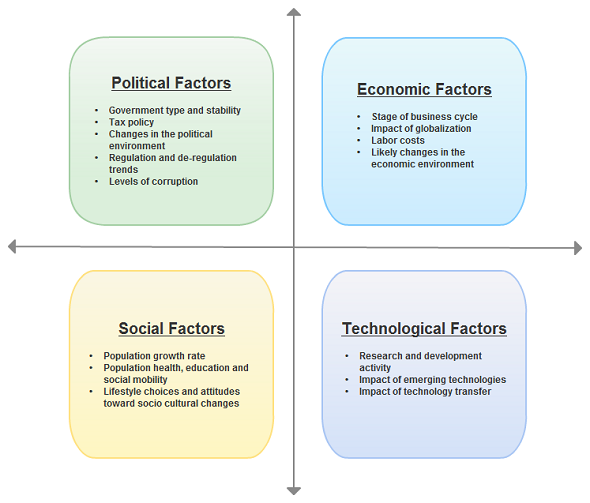
\includegraphics[height=7.5cm]{../pics/PEST}
	\end{figure}
}

\frame{
	\frametitle{The External View}
	\framesubtitle{BCG Matrix (Source: \href{http://www.managementstudyguide.com/bcg-matrix.htm}{Management Study Guide})} 
	\begin{figure}
	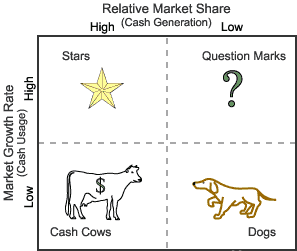
\includegraphics[height=5cm]{../pics/bcgmatrix}
	\end{figure}
}

\frame{
	\frametitle{The External View}
	\framesubtitle{Porter 5 Forces (Art by Denis Fadeev [\href{http://creativecommons.org/licenses/by-sa/3.0}{CC BY-SA 3.0}], via Wikimedia Commons)}
	\begin{figure}
	
\includegraphics[height=7.5cm]{../pics/Porter-5-forces}
	\end{figure}
}

\frame{
	\frametitle{The External View}
	\framesubtitle{A 6$^{th}$ force to Porter's model}
	\begin{block}{Bargaining Power of Complements}
		Complements have the power to generate network externalities and winner-take-all markets. Their bargaining power can influence an industry's competitive environment. The more differentiated and rare, the more power. The more commoditized and in excess capacity, the less power (e.g. IBM PC and Windows OS).
	\end{block}
}

\frame{
	\frametitle{The External View}
	\framesubtitle{Key Success Factors to gain Competitive Advantage}
	\begin{itemize}
		\item Firms compete for a share of the industry pie:
		\pause
		\begin{itemize}
			\item What do customers want? (Demand side)
			\pause
			\item What does the firm need to do to survive competition? (Competition on the Supply side)
		\end{itemize}
		\pause
		\item Key Success Factors: derive from the above two
	\end{itemize}
}

\frame{
	\frametitle{The External View}
	\framesubtitle{Examples of Key Success Factors to gain Competitive Advantage (\cite{grant2006})} 
	\begin{table}\fontsize{5}{6}\selectfont %\tiny
	\begin{tabular}{p{1cm} p{3cm} p{3.5cm} p{3cm}}
	\toprule
	{} & {\tiny\textbf{What do Customers want?}} & {\tiny\textbf{How do Firms survive competition?}} & {\tiny\textbf{Key Sucess Factors}} \\
	\midrule
	Steel & 
		\begin{itemize}
		\item Low price
		\item Product consistency
		\item Reliability of supply
		\item Specific technical specs
		\end{itemize} &
		\begin{itemize}
			\item Commodity products, excess capacity, high fixed costs, exit barriers, and substitute competition mean intense price competition and cyclical profitability
			\item Cost efficiency and strong financial resources are essential
		\end{itemize} &
		\begin{itemize}
			\item Conventional sources of cost efficiency include: large-scale plants, low-cost locations, rapid adjustment of capacity to output
			\item Alternatively, high technology, small scale plants can achieve low costs through flexibility and high productivity
			\item Differentiation through technical specifications and service quality 
		\end{itemize} \\
	Fashion clothing & 
		\begin{itemize}
			\item Wide variety of customerpreferences relating to garment type, style, quality, colour
			\item Customers willing to pay price premium for brand, stylishness, exclusivity, and quality
			\item Mass market highly price sensitive
		\end{itemize} &
		\begin{itemize}
			\item Low barriers to entry and exit, low seller concentration, and buying power of retail chains imply intense competition
			\item Differentiation can yield substantial price premium, ubt imitation is rapid
		\end{itemize} & 
		\begin{itemize}
			\item Need to combine effective differentiation with low costs
			\item Key differentiation variables are speed of response to changing high fashions, style, reputation, and quality
			\item Cost eficiency requires manufacture in low wage countries
		\end{itemize} \\
	\midrule
	\bottomrule
	\end{tabular}
	\end{table}
}

\frame{
	\frametitle{The External View}
	\framesubtitle{Examples of Key Success Factors to gain Competitive Advantage (\cite{grant2006})} 
	\begin{table}\fontsize{5}{6}\selectfont %\tiny
	\begin{tabular}{p{1cm} p{3cm} p{3.5cm} p{3cm}}
	\toprule
	{} & {\tiny\textbf{What do Customers want?}} & {\tiny\textbf{How do Firms survive competition?}} & {\tiny\textbf{Key Sucess Factors}} \\
	\midrule
	Supermarkets & 
		\begin{itemize}
			\item Low prices
			\item Convenient location
			\item Wide range of products adapted to local preferences
			\item Fresh/quality produce; good service; ease of parking; pleasant ambiance
		\end{itemize} & 
		\begin{itemize}
			\item Markets localized
			\item Intensity of price competition depends on number and proximity of competitors
			\item Bargaining power is a critical determinant of cost of bought-in goods
		\end{itemize} &
		\begin{itemize}
			\item Low-cost operation requires operational efficiency, scale-efficient stores, large aggregate purchases to maximize buying power, low wage costs
			\item Differentiation requires large stores (to allow wide product range), convenient location, easy parking
		\end{itemize} \\
	\midrule
	\bottomrule
	\end{tabular}
	\end{table}
}

\frame{
	\frametitle{The External View}
	\framesubtitle{Exercise}
	\begin{alertblock}{Industry Analysis}
		Analyse the industry that focuses on IT systems addressing the 8 business functions that we'll be studying in this course. Select the top 2 competitors and explain their strategy, as well as Odoo SA's (the editor of Odoo).
	\end{alertblock}
}

% --------------------- Internal View --------------------------
\subsection{The Internal View (be the best)}
\begin{frame}[c]{The Internal View}
	\centering
	\Huge{How to build and maintain a competitive advantage?}
\end{frame}

\frame{
	\frametitle{The Internal View}
	\framesubtitle{Leveraging Internal Resources \& Capabilities}
	\begin{itemize}
		\item Select a strategy that leverages a firm's key strengths (e.g. Kodak)
		\pause
		\item Develop its resources \& capabilities (e.g. WIPRO)
	\end{itemize}
}

\frame{
	\frametitle{The Internal View}
	\framesubtitle{Resources $\neq$ Capabilities (\cite{grant2006})}
	\begin{figure}
	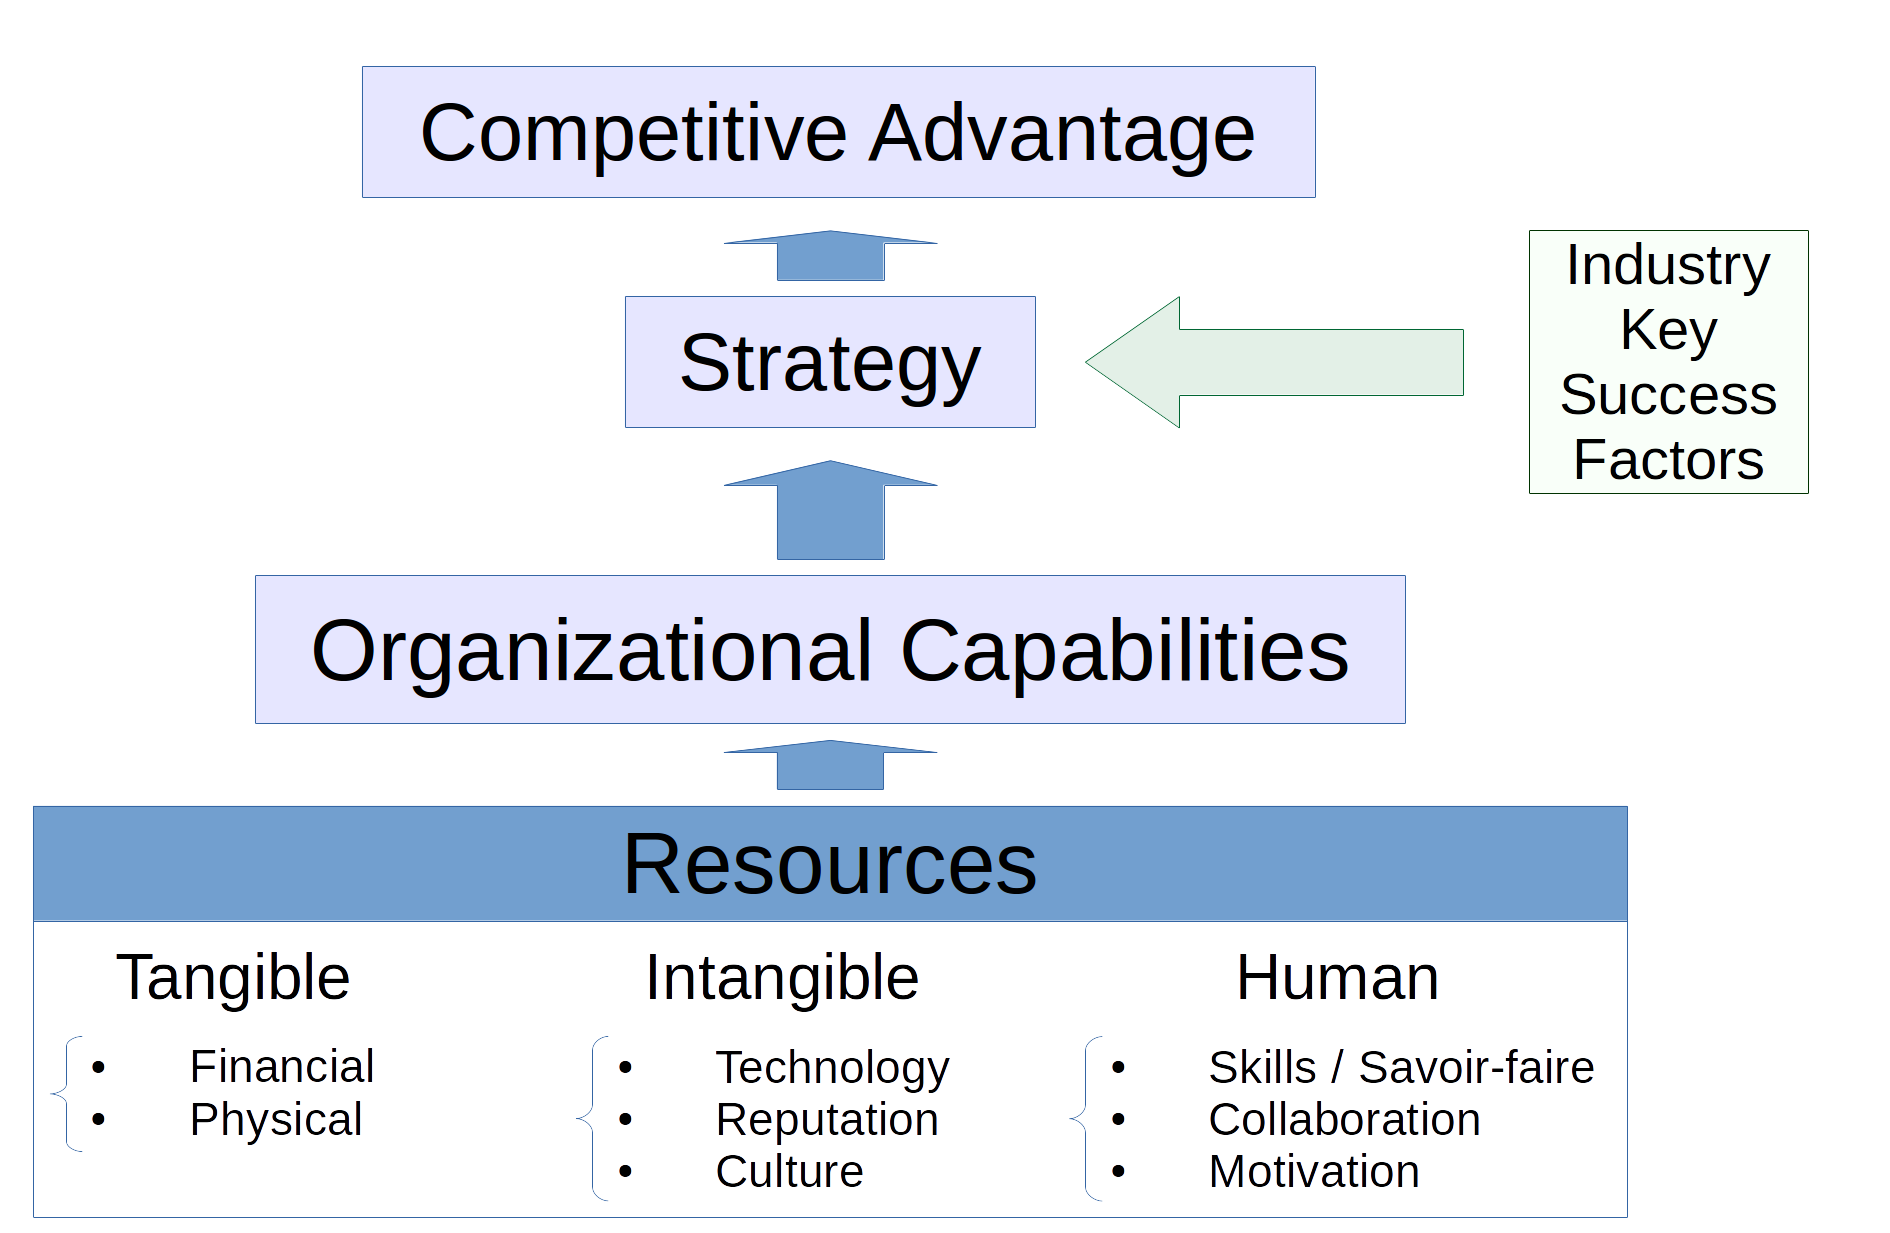
\includegraphics[height=7.5cm]{../pics/grant-link-resources-and-capabilities-with-competitive-advantage}
	\end{figure}
}

\frame{
	\frametitle{The Internal View}
	\framesubtitle{Some Resources ($\neq$ Capabilities) (\cite{grant2006})}
	\begin{table}\fontsize{5}{6}\selectfont %\tiny
	\begin{tabular}{p{2cm} p{6cm} p{3cm}}
	\toprule
	{\tiny\textbf{Tangible Resources}} & {\tiny\textbf{Characteristics}} & {\tiny\textbf{Key Indicators}} \\
	\midrule
%	\multicolumn{3}{l}{Tangible Resources}\\
	Financial Resources & Firm's borrowing capacity and internal funds generation determining its capacity for investment & 
		\begin{itemize}
			\item Debt/Equity ratio
			\item Operating Cash Flow
			\item Credit Rating
		\end{itemize} \\
	Physical Resources & Constrain the firm's set of production possibilities and impact its cost position. Key characteristics include:
		\begin{itemize}
			\item size, location, technical sophistication, and flexibility of plant and equipment
			\item location and alternative uses for land and buildings
			\item reserves of raw materials
		\end{itemize} &
		\begin{itemize}
			\item Market values of fixed assets
			\item Vintage of capital equipment
			\item Scale of plants
			\item Flexibility of fixed assets
		\end{itemize} \\
	\midrule
	\bottomrule
	\end{tabular}
	\end{table}
}

\frame{
	\frametitle{The Internal View}
	\framesubtitle{Some Resources ($\neq$ Capabilities) (\cite{grant2006})}
	\begin{table}\fontsize{5}{6}\selectfont %\tiny
	\begin{tabular}{p{2cm} p{5cm} p{4cm}}
	\toprule
	{\tiny\textbf{Intangible Resources}} & {\tiny\textbf{Characteristics}} & {\tiny\textbf{Key Indicators}} \\
	\midrule
%	\multicolumn{3}{l}{Intangible Resources}\\
	Technological Resources & 
		\begin{itemize}
			\item Intellectual property, patent portfolio, copyright, trade secrets
			\item Resources for innovation: research facilities, technical and scientific employees
		\end{itemize} &
		\begin{itemize}
			\item Number and significance of patents
			\item Revenue from licensing patents and copyright
			\item R\&D staff as a percentage of total employment
			\item Number and location of research facilities
		\end{itemize} \\
	Reputation & 
		\begin{itemize}
			\item Reputation with customers through the ownership of brands and trademarks; established relationships with customers; the reputation of the firm's produts and services for quality and reliability
			\item The reputation of the company with suppliers, government, and the community
		\end{itemize} &
		\begin{itemize}
			\item Brand recognition
			\item Brand equity
			\item Percentage of repeat buying
			\item Objective measures of comparative product performance (e.g. J.D. Power ratings)
			\item Surveys of corporate reputation (e.g. \emph{Fortune})
		\end{itemize} \\
	\midrule
	\bottomrule
	\end{tabular}
	\end{table}
}

\frame{
	\frametitle{The Internal View}
	\framesubtitle{Some Resources ($\neq$ Capabilities) (\cite{grant2006})}
	\begin{table}\fontsize{5}{6}\selectfont %\tiny
	\begin{tabular}{p{2cm} p{5cm} p{4cm}}
	\toprule
	{\tiny\textbf{Human Resources}} & {\tiny\textbf{Characteristics}} & {\tiny\textbf{Key Indicators}} \\
	\midrule
	{} &	\begin{itemize}
			\item The education, training and experiences of employees determine the skills available to the firm
			\item The adaptability of employees contributes to the strategic flexibility of the firm. The social and collaborative skills of employees determine the capacity of the firm to transform human resources into organizational capabilities.
			\item the commitment and loyalty of employees determine the capacity of the firm to attain and maintain competitive advantage
		\end{itemize} &
		\begin{itemize}
			\item Educational, technical, and porfessional qualifications of employees
			\item Copmensation relative to industry
			\item Percentage of days lost through stoppages and industrial disputes
			\item Absentee rates
			\item Employee turnover rates
		\end{itemize} \\
	\midrule
	\bottomrule
	\end{tabular}
	\end{table}
}

\frame{
	\frametitle{The Internal View}
	\framesubtitle{Maslow's Hierarchy of Needs (Art by FireflySixtySeven [\href{http://creativecommons.org/licenses/by-sa/4.0}{CC BY-SA 4.0}], via Wikimedia Commons)}
	\begin{figure}
	\includegraphics[height=7.5cm]{../pics/MaslowsHierarchyOfNeeds}
	\end{figure}
}

\frame{
	\frametitle{The Internal View}
	\framesubtitle{Porter Value Chain Analysis (Art by Dinesh Pratap Singh [\href{http://creativecommons.org/licenses/by-sa/3.0}{CC BY-SA 3.0}], via Wikimedia Commons)}
	\begin{figure}
	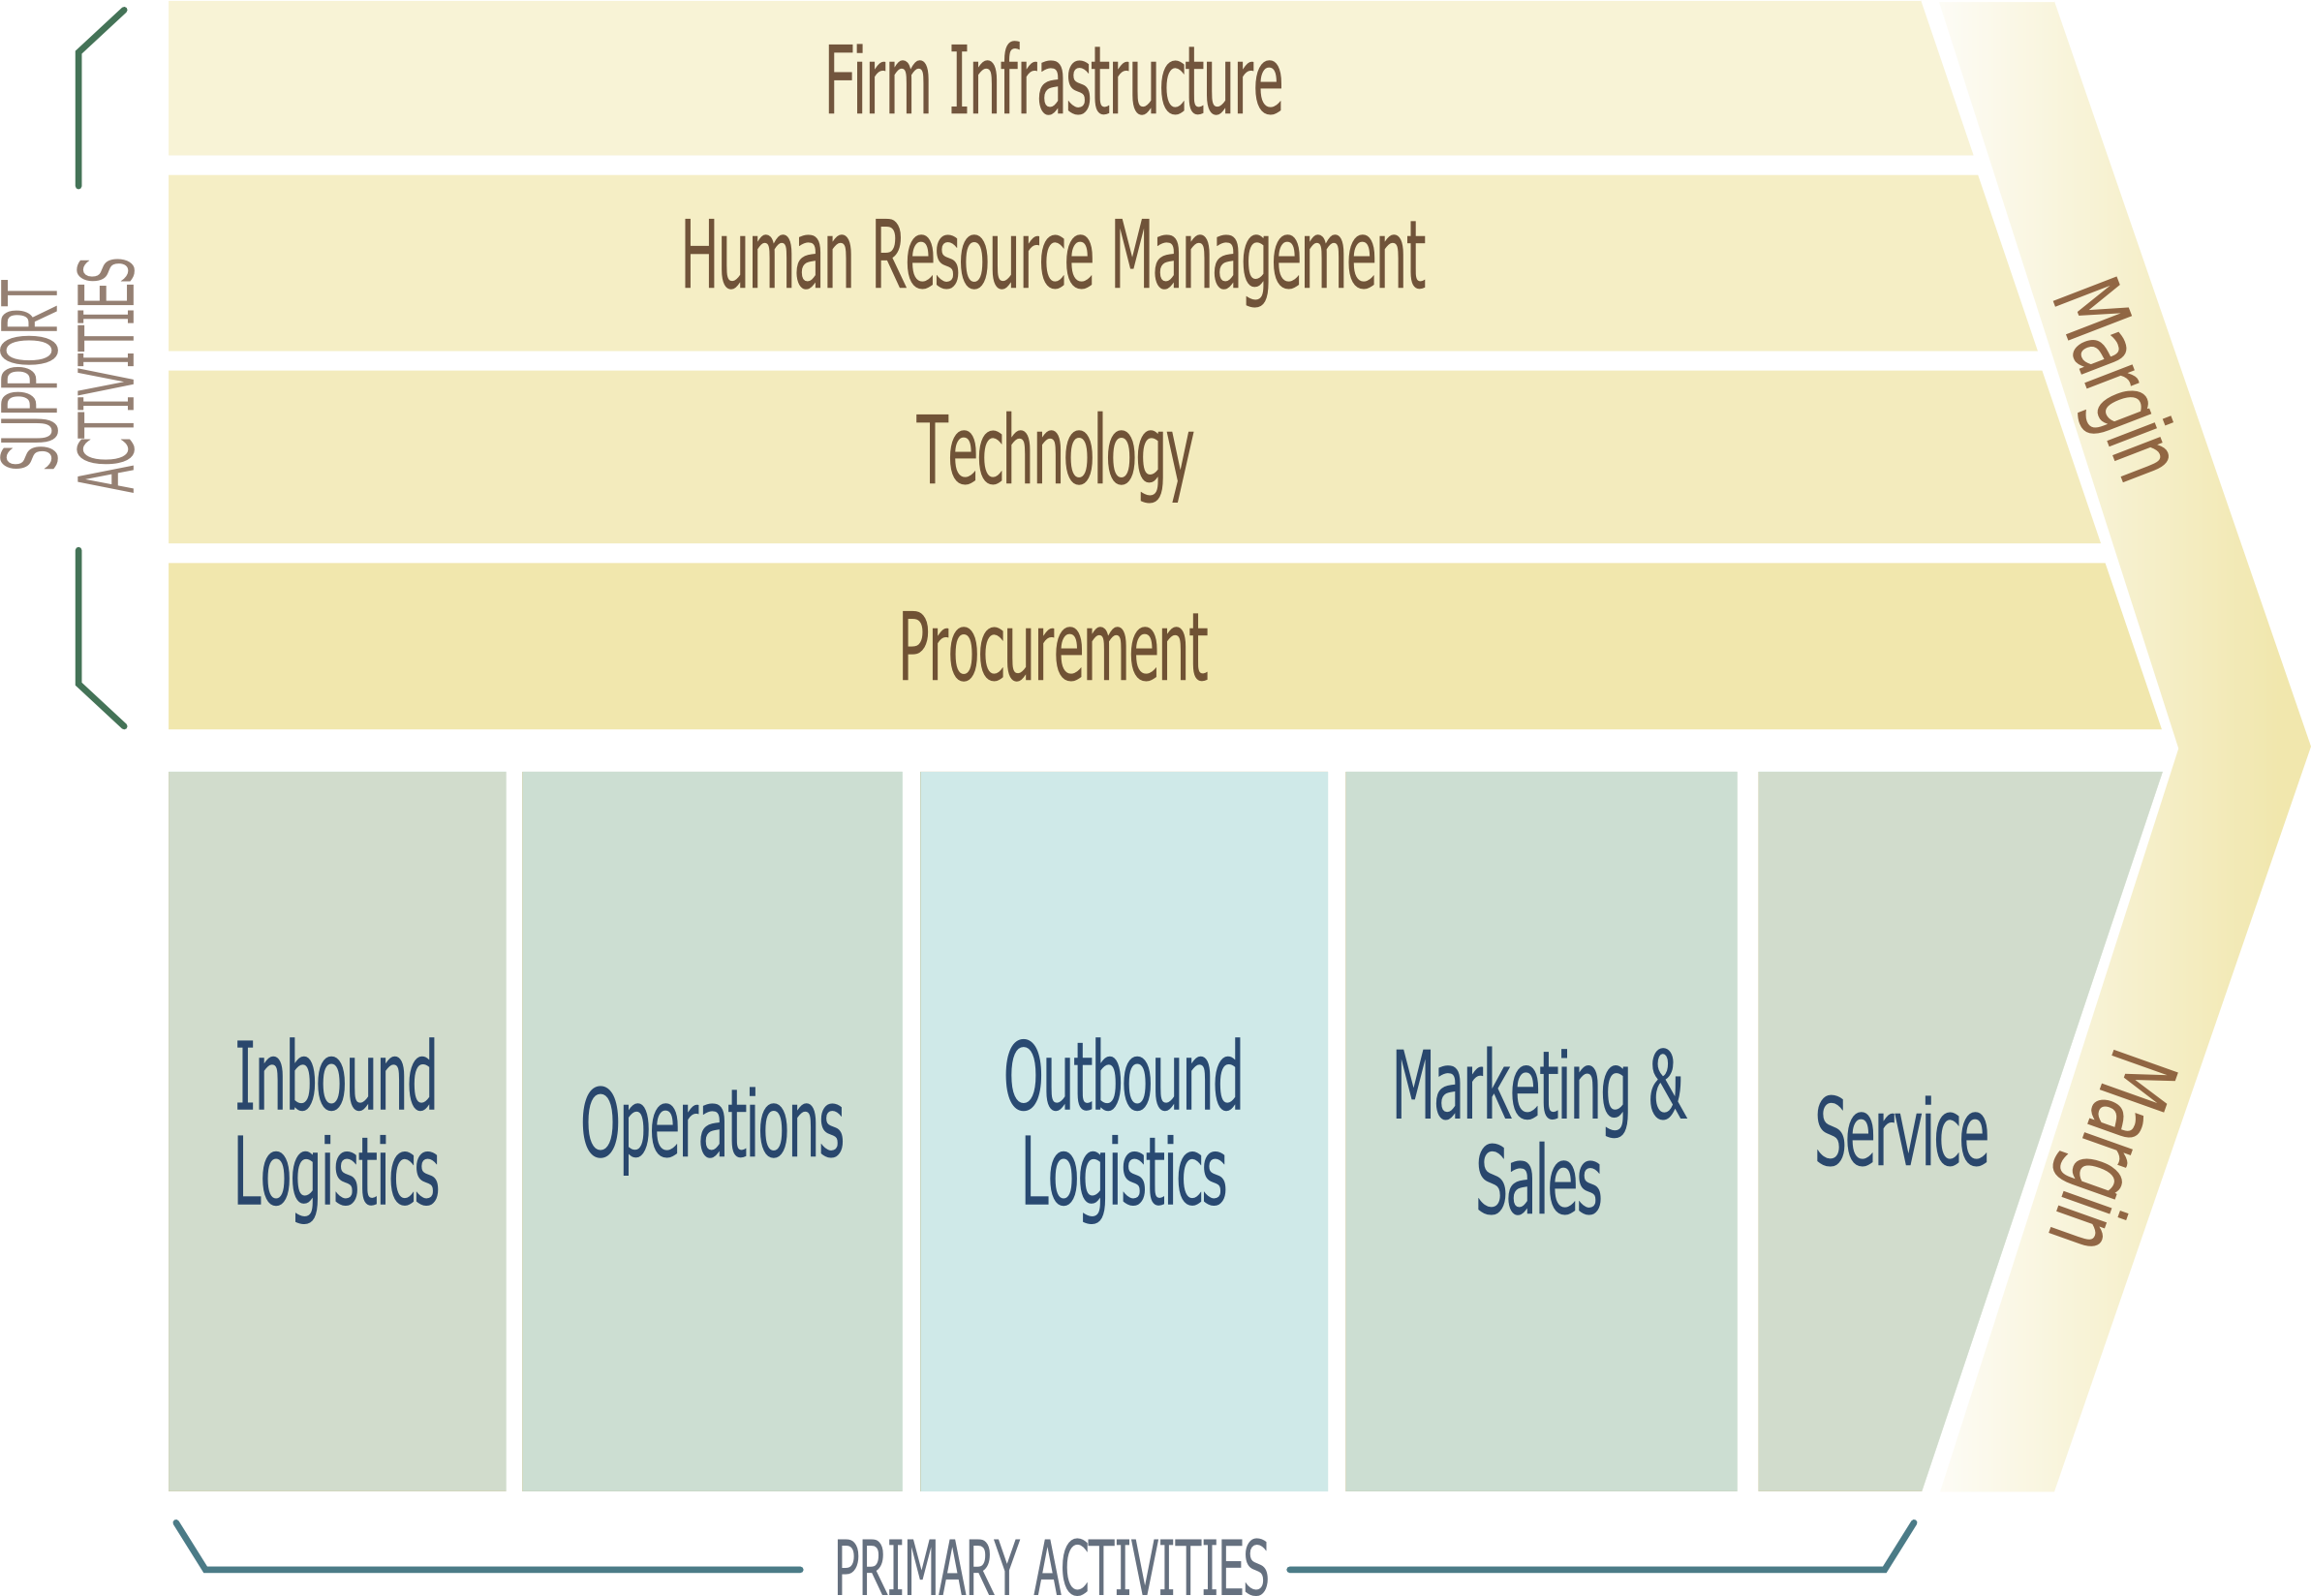
\includegraphics[height=6.5cm]{../pics/Porter_Value_Chain}
	\end{figure}
}
% TODO add slides with pics about the learning experience curve decreasing the cost of producing goods and services

\frame{
	\frametitle{The Internal View}
	\framesubtitle{Rent-Earning Potential of Resources \& Capabilities (\cite{grant2006})}
	\begin{figure}
	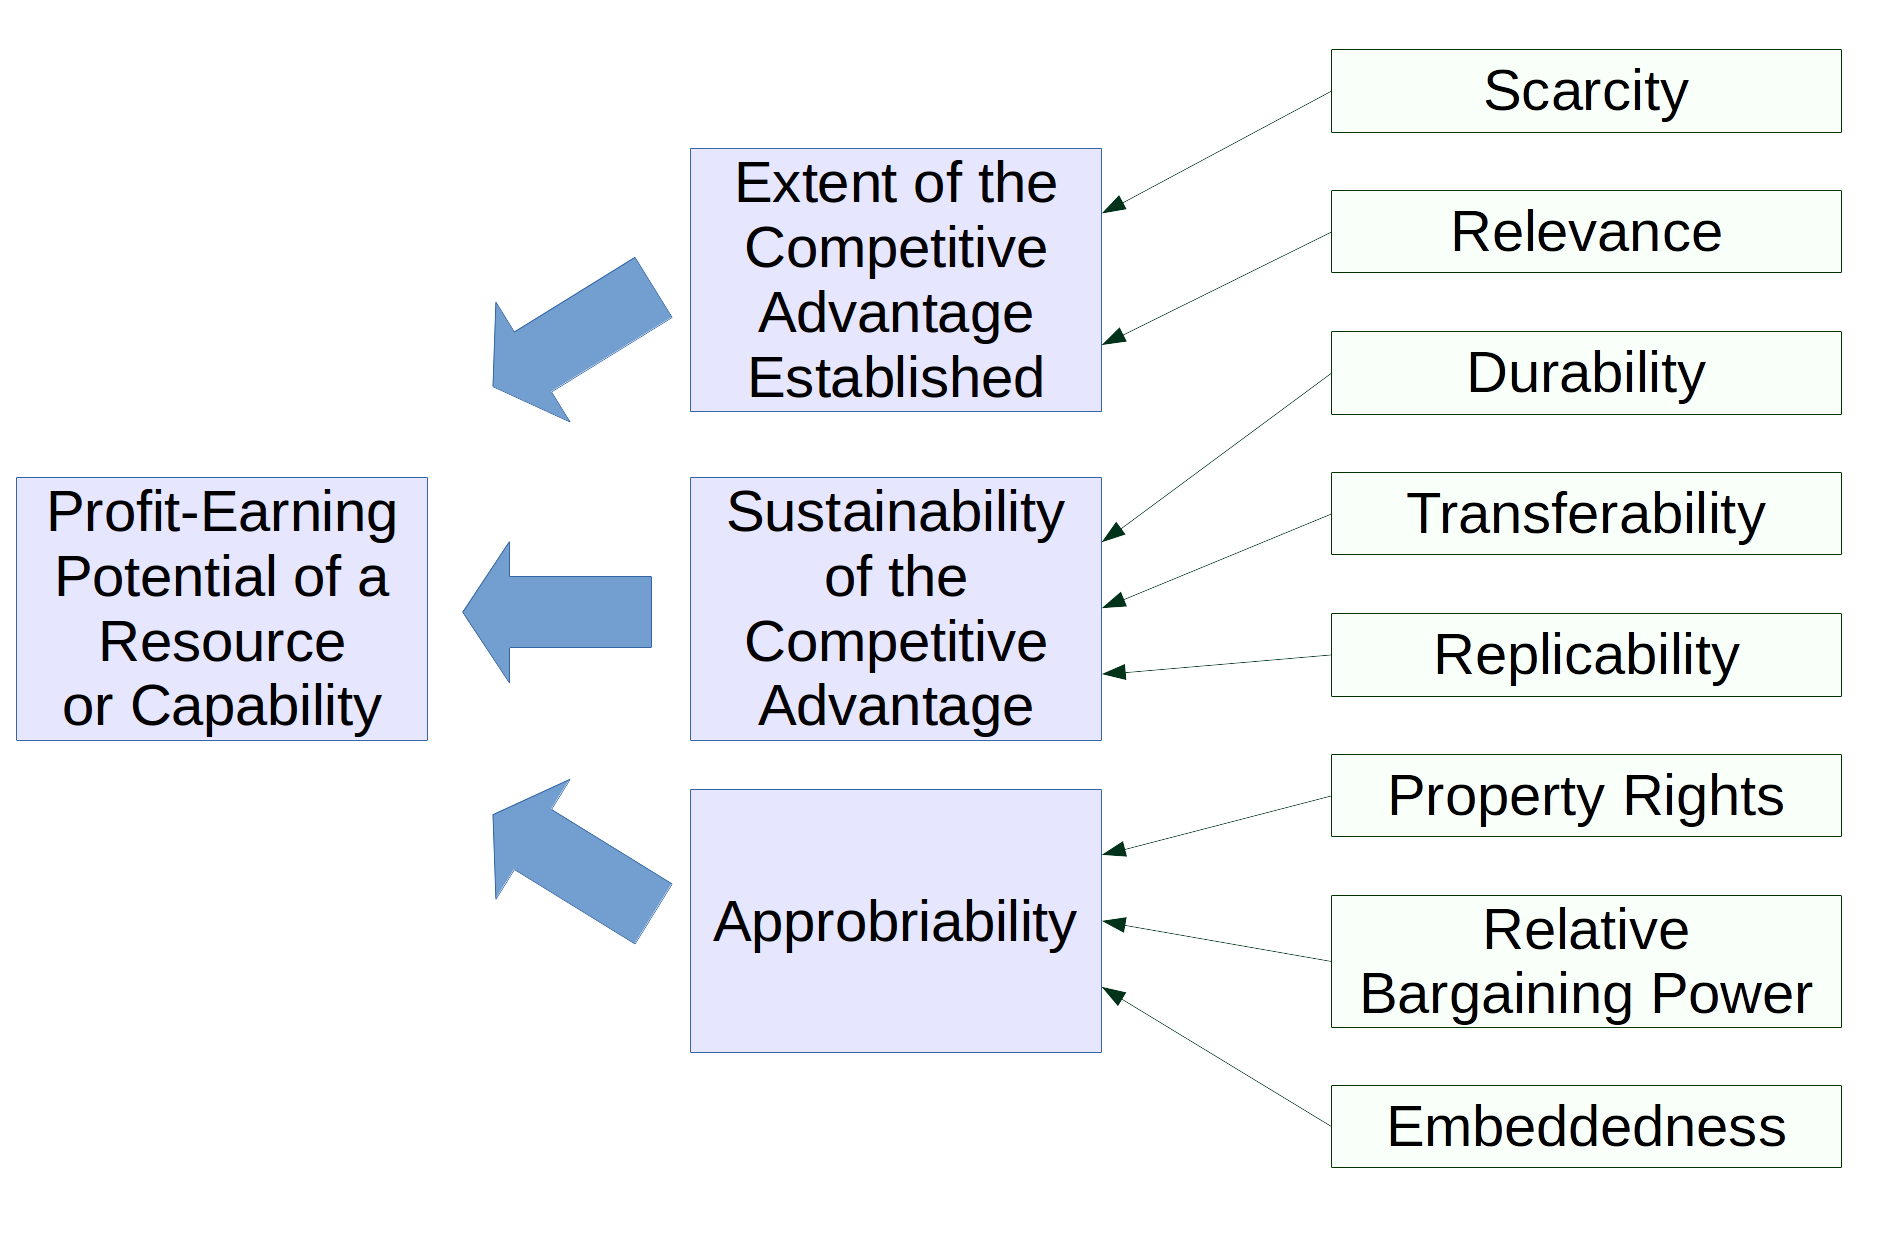
\includegraphics[height=7.5cm]{../pics/grant-rent-earning-potential.png}
	\end{figure}
}

\frame{
	\frametitle{The Internal View}
	\framesubtitle{Practical Steps}
	\begin{enumerate}
		\item Identify key resources \& capabilities
		\begin{enumerate}
			\item Start by identifying the key success factors (demand side)
			\item Identify which resources and capabilities are mobilized in relations to these
			\item Identify the capabilities in the company's value chain and which resources they draw from (supply side)
		\end{enumerate}
		\item Estimate resources \& capabilities across two dimensions:
			\begin{enumerate}
				\item importance
				\item strength
			\end{enumerate}
		\item Develop strategy implications
			\begin{enumerate}
				\item Exploit key strengths
				\item Manage key weaknesses
				\item Deal with superfluous strengths
			\end{enumerate}
		\item Build \& Strengthen resources and capabilities
	\end{enumerate}
}

\frame{
	\frametitle{The Internal View}
	\framesubtitle{VW as an hypotetical Example --Part 1: Resources (\cite{grant2006})}
	\begin{table}\fontsize{5}{6}\selectfont %\tiny
	\begin{tabular}{p{2cm} C{2cm} C{2cm} p{4cm}}
	\toprule
	{\tiny\textbf{Resources}} & {\tiny\textbf{Importance}} & {\tiny\textbf{VW's Strength}} & {\tiny\textbf{Comments}} \\
	\midrule
	R1. Finance & 6 & 4 & VW's capital investment exceeds operating cash flows. Deb/equity ratio is high compared to the industry \\
	R2. Technology & 7 & 5 & Despite technical strengths, VW is not a leader in automotive technology \\
	R3. Plant and equipment & 8 & 8 & Has invested heavily in upgrading plants\\
	R4. Location & 7 & 4 & Plants in low cost, growth markets (China, Mexico), but German manufacturing base is very high cost\\
	R5. Distribution (dealership network) & 8 & 5 & Geographically extensive distribution with special strengh in emerging markets. Historically weak in the US.\\
	\midrule
	\bottomrule
	\end{tabular}
	\end{table}
}

\frame{
	\frametitle{The Internal View}
	\framesubtitle{VW as an hypotetical Example --Part 2: Capabilities (\cite{grant2006})}
	\begin{table}\fontsize{5}{6}\selectfont %\tiny
	\begin{tabular}{p{2cm} C{2cm} C{2cm} p{4cm}}
	\toprule
	{\tiny\textbf{Capabilities}} & {\tiny\textbf{Importance}} & {\tiny\textbf{VW's Strength}} & {\tiny\textbf{Comments}} \\
	\midrule
	C1. Product development & 7 & 5 & Traditionnally weak at VW. Major hits are few (e.g. Beetle in 1938, Golf in 1974). Despite recent upgrading, results are still low compared to Toyota. \\
	C2. Purchasing & 7 & 5 & Traditionnaly weak --strengthened by senior hires from Opel and elsewhere.\\
	C3. Engineering & 7 & 9 & The core technical strength of VW.\\
	C4. Manufacturing & 8 & 7 & Problems of inflexibility, and indifferent quality largely resolved during the 90s.\\
	C5. Financial management & 6 & 3 & Has traditionally lacked a strong financial orientation.\\
	C6. R\&D & 6 & 4 & A comparative strength of VW but becoming less important as technology shifts increasingly to suppliers.\\
	C7. Marketing and sales & 9 & 4 & Despite traditional weakness in recognizing and meeting customer needs in different national markets, VW has increased its sensitivity to the market, improved brand management and managed its advertising and promotion with increasing dexterity.\\
	C8. Government relations & 4 & 8 & Important in emerging markets.\\
	\midrule
	\bottomrule
	\end{tabular}
	\end{table}
}

\frame{
	\frametitle{The Internal View}
	\framesubtitle{Sample Appraisal (\cite{grant2006})}
	\begin{figure}
	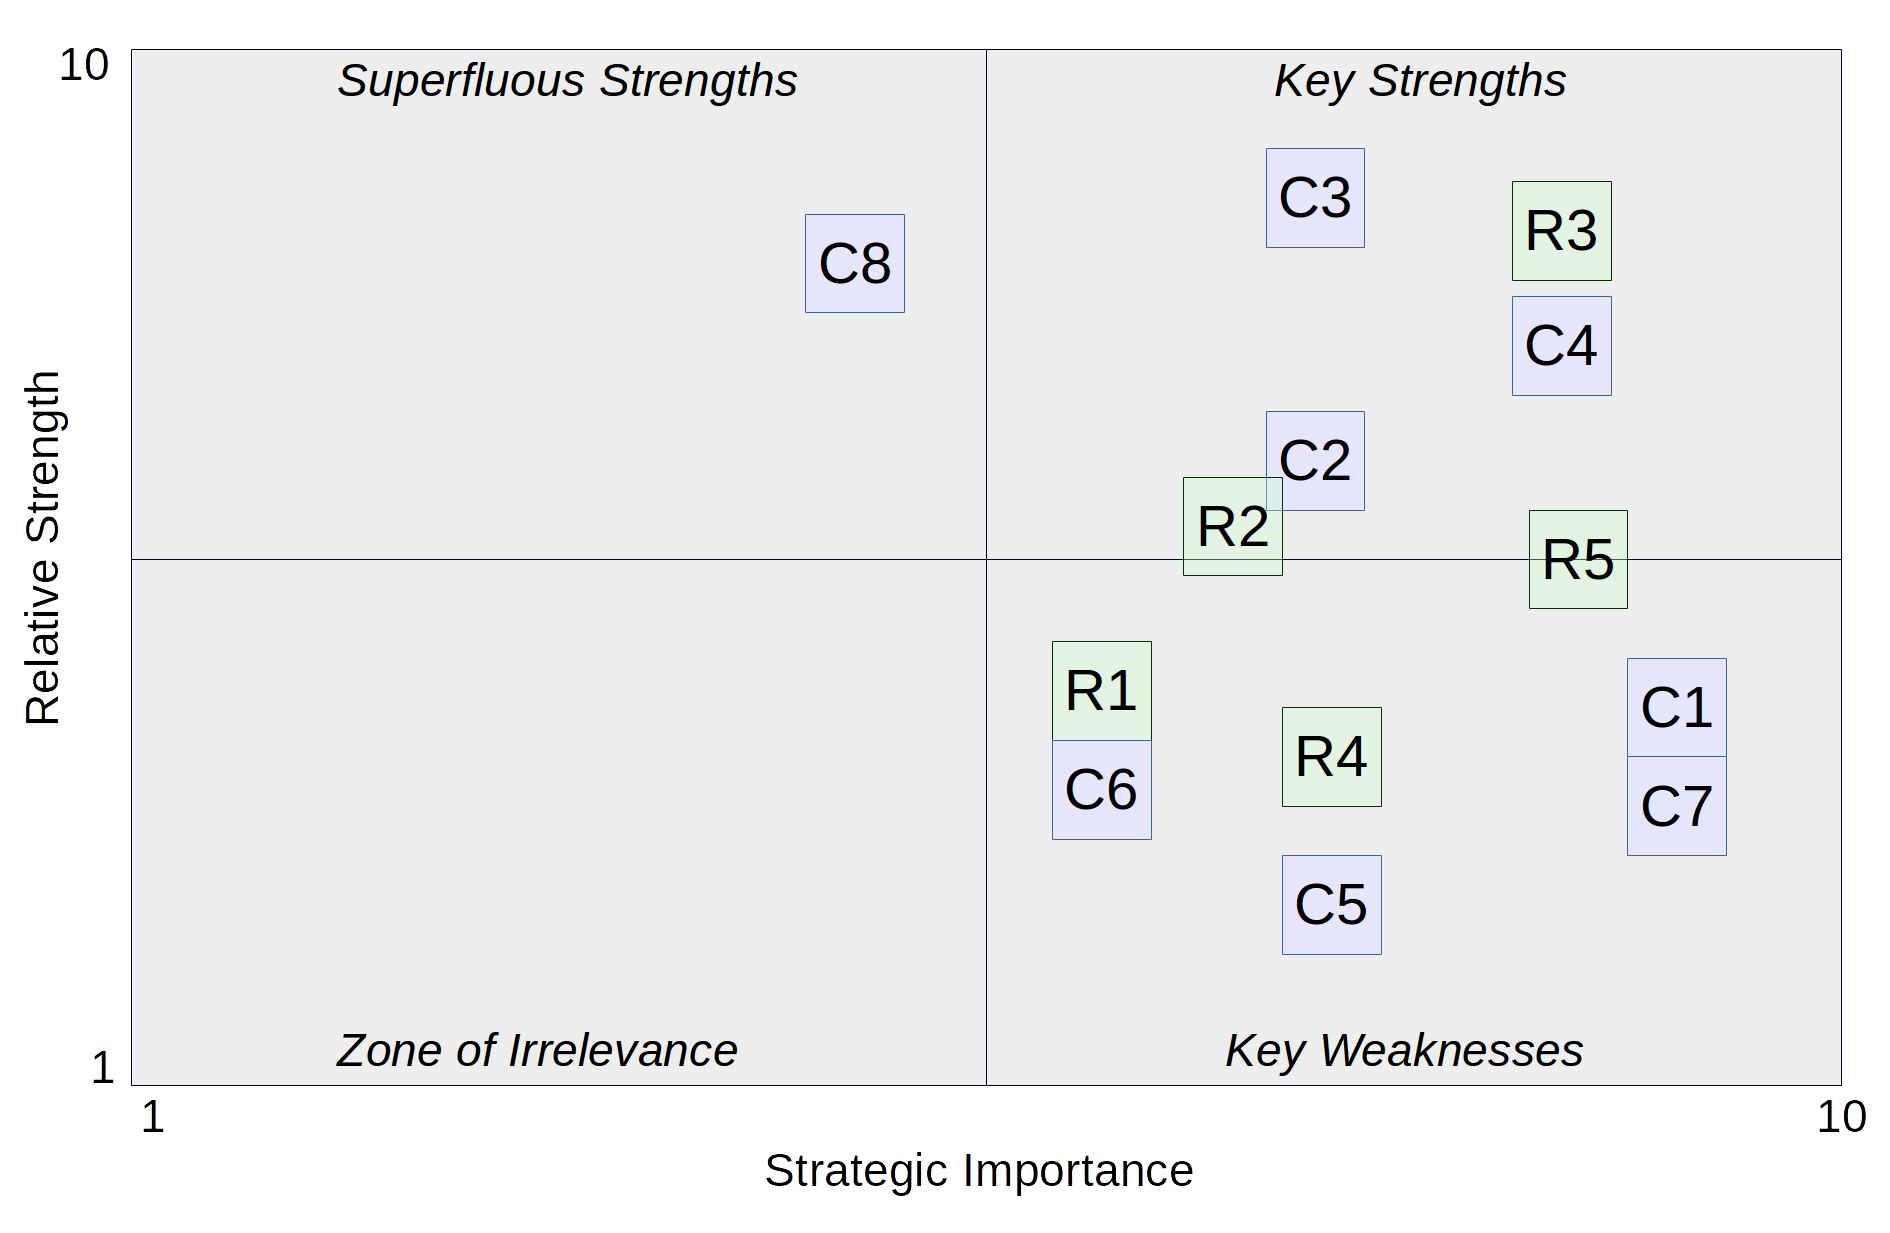
\includegraphics[height=7.5cm]{../pics/grant-appraisal.png}
	\end{figure}
}
% TODO make an example

% --------------------- Competitive Strategies --------------------------
\subsection{Competitive Strategies}
\begin{frame}[c]{Competitive Strategies}
	\centering
	\Huge{How to play the game?}
\end{frame}

\frame{
	\frametitle{Competitive Strategies}
	\framesubtitle{Porter's Generic Strategies}
	\begin{figure}
	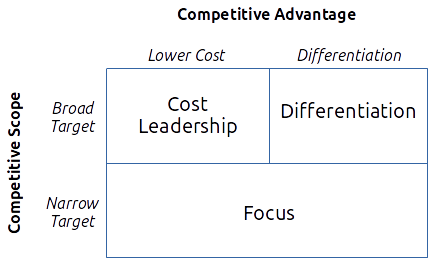
\includegraphics[height=6cm]{../pics/porter-generic-strategies2}
	\end{figure}
}
% TODO add more slides with examples (companies with their strategies)

\frame{
	\frametitle{The Internal View}
	\framesubtitle{Strategy --the Big Picture (\cite{mintzberg2008strategy})}
	\begin{figure}
	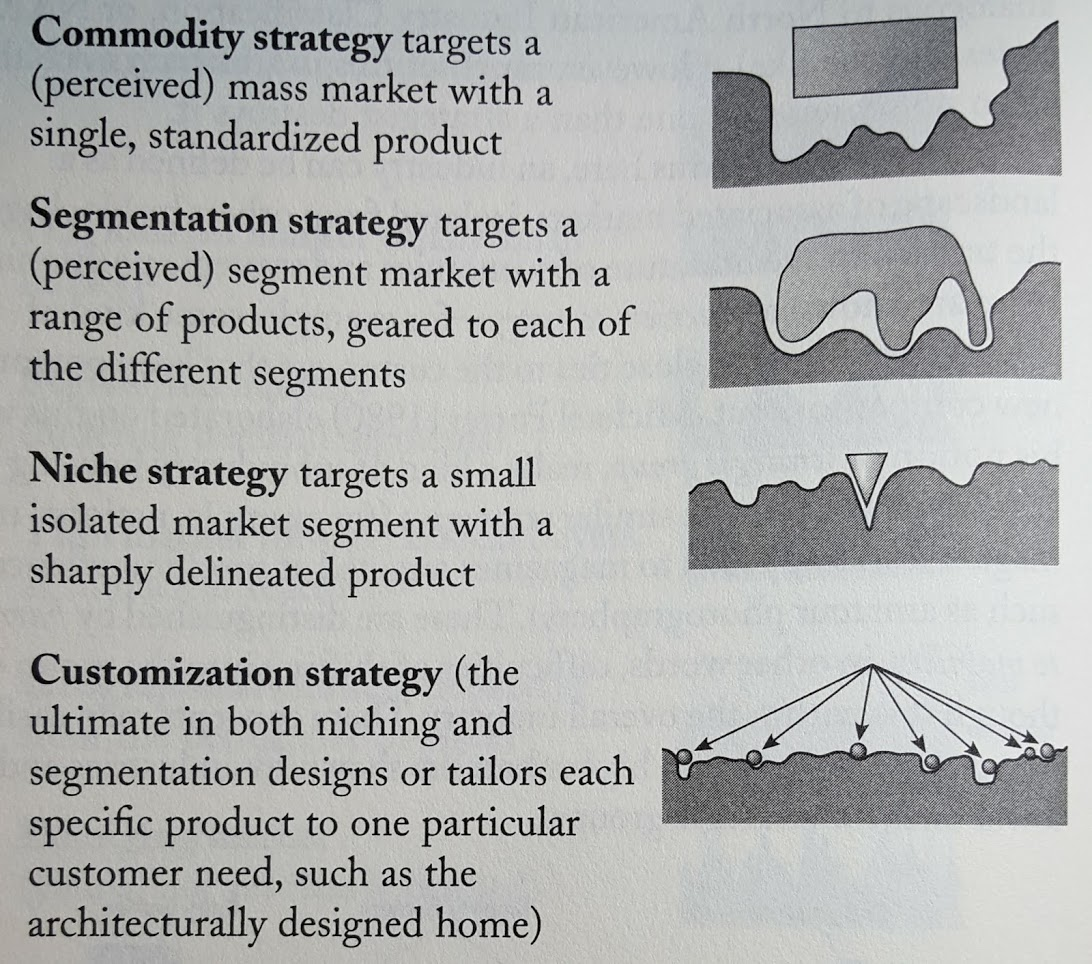
\includegraphics[height=7.5cm]{../pics/mintzberg-main-strategies}
	\end{figure}
}

% ~ ~ ~ References
\frame{
	\frametitle{Introduction to Strategy}
	\framesubtitle{References}
	% keyword refers to bib file: references-KEYWORD.bib, and to the Tex file: section-KEYWORD.tex
	\url{http://valuebasedmanagement.net}\\
	\url{http://www.real.gold.ac.uk/essayguide/index.html}\\
	\printbibliography[keyword=strategy-intro]
}



% Afternoon: Thinking Strategically
% 1st: micro, then macro
%% (C) Marc Lijour, 2016-2017 
% Licensed under a Creative Commons License BY-SA
% https://creativecommons.org/licenses/by-sa/2.5/ca/
% Presentation for the Small Business Digitization Initiative (SBDI) training program
% see http://www.ictc-ctic.ca/small-business-digitization-initiative/ 
% authored by Marc Lijour, December 2016
% for the session running from January 2017 to September 2017
% 
% ======================================================================================================
%                                   GLOBAL COMPETITION - MACROECONOMIC FORCES
% ======================================================================================================
\section{Global Competition}
% --------------------- Currencies --------------------------
\subsection{Currency Competition}
\frame{
	\frametitle{Global Competition}
	\framesubtitle{Purchasing Power Parity (PPP)}
	\begin{itemize}
		\item Idea that a basket of common goods would have the same pricing value across countries and currencies
		\pause
		\item Assumptions:
			\begin{itemize}
				\item no transaction cost (currency exchange)
		\pause
				\item no trade barriers
			\end{itemize}
		\pause
		\item Useful to think about:
			\begin{itemize}
				\item Arbitrage
		\pause
				\item Undervaluation and overvaluation due to market expectation (e.g. US President Trump \& Mexico)
		\pause
				\item Policies such as currency fluctuation and trade barriers
			\end{itemize}
	\end{itemize}
}

% From the Economist:
% THE Big Mac index was invented by The Economist in 1986 as a lighthearted guide to whether currencies are at their “correct” level. It is based on the theory of purchasing-power parity (PPP), the notion that in the long run exchange rates should move towards the rate that would equalise the prices of an identical basket of goods and services (in this case, a burger) in any two countries. For example, the average price of a Big Mac in America in January 2017 was $5.06; in China it was only $2.83 at market exchange rates. So the ``raw'' Big Mac index says that the yuan was undervalued by 44% at that time. 
\frame{
	\frametitle{Global Competition}
	\framesubtitle{Currency Valuation: \href{http://www.economist.com/content/big-mac-index}{The Big Mac Index (\cite{bigmacindex})}}
	%\framesubtitle{Currency Valuation: \href{http://www.economist.com/content/big-mac-index}{The Big Mac Index}}
	% Discuss: it does not take into account labor cost
	\begin{figure}
	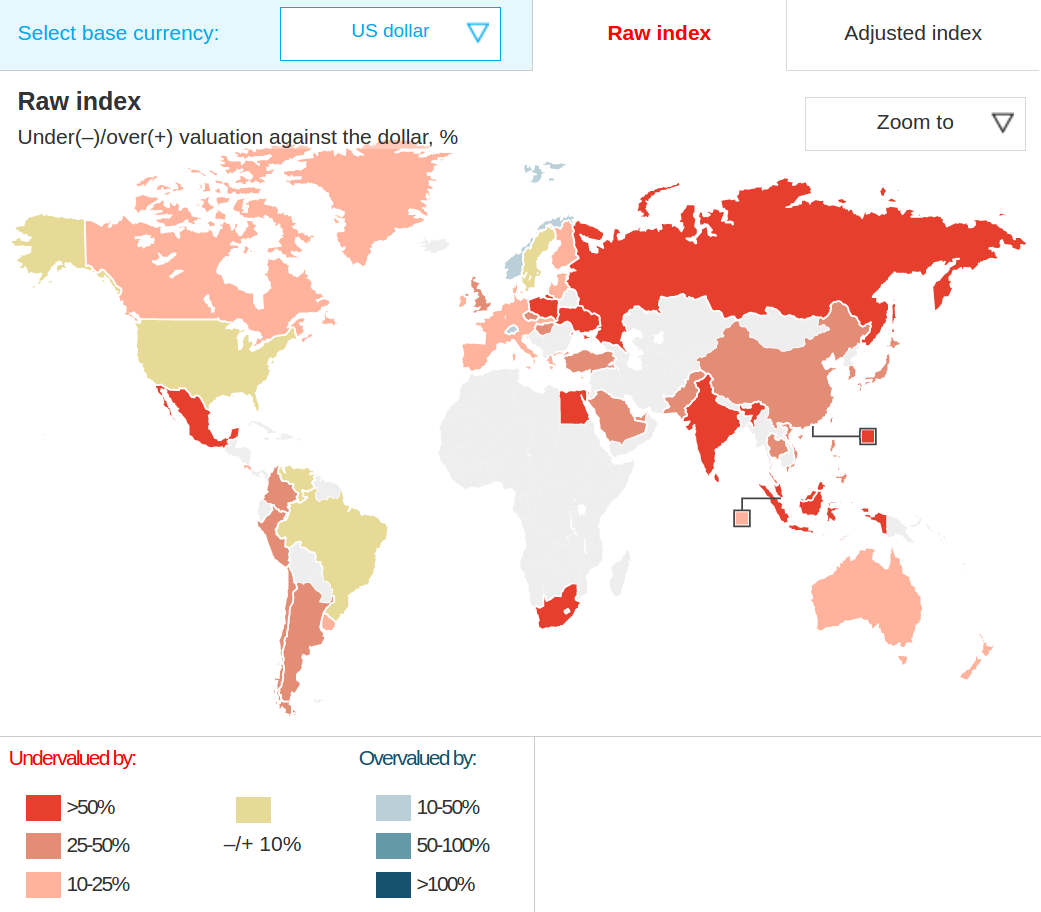
\includegraphics[height=7.5cm]{../pics/big-mac-index}
	\end{figure}
}

% --------------------- Trade Barriers --------------------------
\subsection{Trade Barriers}
\frame{
	\frametitle{Global Competition}
	\framesubtitle{Tariffs}
	\begin{itemize}
		\item Tax on the circulation of goods
		\pause
	\item See Canada's \href{http://www.cbsa-asfc.gc.ca/trade-commerce/tariff-tarif/2017/menu-eng.html}{Customs Tariff (\cite{customstariff2017})}
		\pause
		\item Countries set their own policies, alone or in association (e.g. NAFTA, TPP, CETA)
		\pause
		\item Policies derive from political viewpoints (changing over time), for example
		\pause
			\begin{itemize}
				\item Canada cuts \$48M in tariffs on food ingredients to boost manufacturing, as \href{http://www.cbc.ca/news/politics/food-ingredient-tariff-cuts-1.3942870}{reported on \citejournal{cbc:foodtariff} (January 20, 2017)}
		\pause
	\item US President Trumps threatened German car makers with a 35\% import tariff, as \href{http://business.financialpost.com/news/transportation/trump-threatens-german-carmakers-with-35-u-s-import-tariff}{reported on the \citejournal{fpost:trumpcar} (January 16, 2017)}
			\end{itemize}
		\pause
		\item Impact on the Manufacturing Industry, Global Supply Chain, Foreign Investment, Currencies\ldots
	\end{itemize}
}

\frame{
	\frametitle{Global Competition}
	\framesubtitle{Non-Tariff Barriers}
	\begin{itemize}
		\item Circulation of staff delivering services across borders
		\pause
		\item Licensing (e.g. cryptography)
		\pause
		\item Standards
		\pause
		\item Quotas
		\pause
		\item Labeling and Packaging conditions
		\pause
		\item Intellectual Property Laws (e.g. patents)
		\pause
		\item Protected Designation of Origin (e.g. Champagne, Feta cheese)
	\end{itemize}
}

\subsection{Fiscal Policies}
\frame{
	\frametitle{Global Competition}
	\framesubtitle{Corporate Tax Rates}
	\begin{figure}
	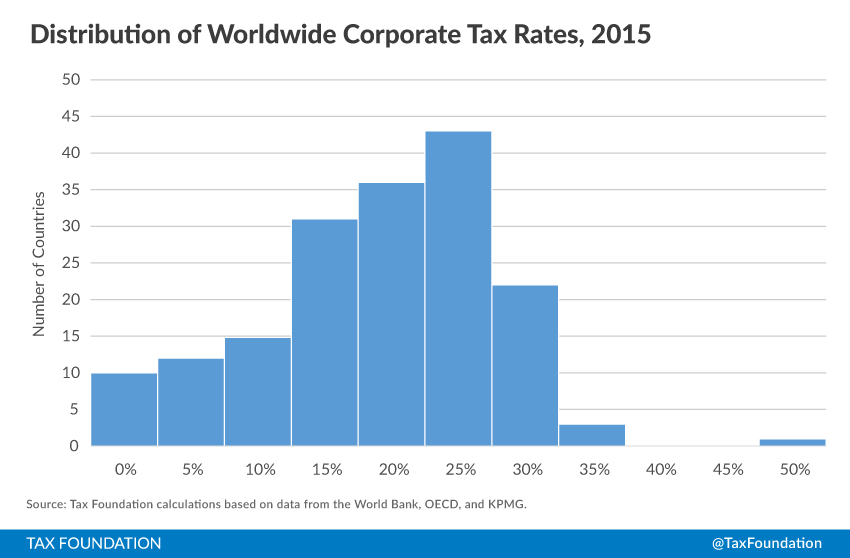
\includegraphics[height=7.5cm]{../pics/taxFoundation2015-worldwide-taxrates}
	\end{figure}
}

\frame{
	\frametitle{Global Competition}
	\framesubtitle{Corporate Income Tax Rates Competition (G7 Top 3 from \href{http://www.investinontario.com/spotlights/canada-ranks-1st-g7-corporate-tax-rate-and-cost-competitiveness}{\cite{kpmg2016}})}
	\begin{figure}
	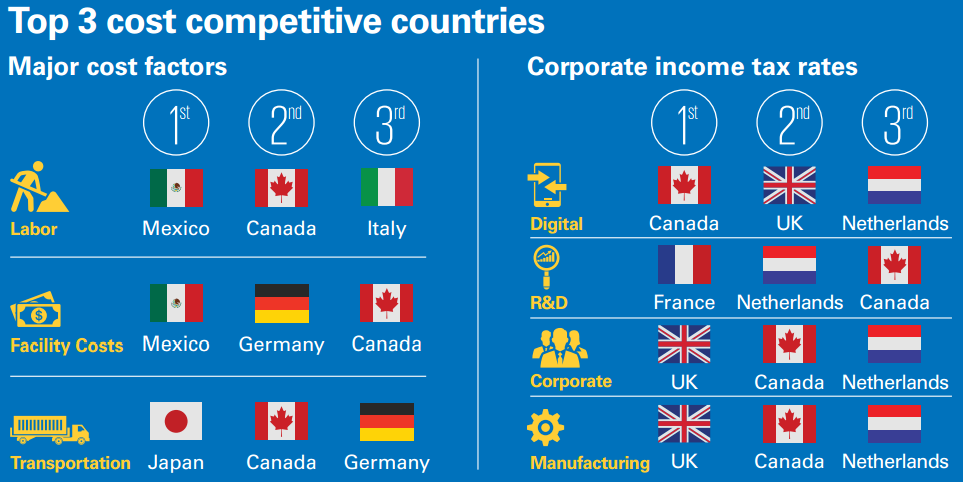
\includegraphics[width=11.5cm]{../pics/KPMG2016-top3-competitive-countries}
	\end{figure}
}

\subsection{Competitiveness Rankings}
\frame{
	\frametitle{Global Competition}
	\framesubtitle{Countries with the lowest business cost (G7 Top 10 from \href{http://www.investinontario.com/spotlights/canada-ranks-1st-g7-corporate-tax-rate-and-cost-competitiveness}{\cite{kpmg2016}})}
	\begin{figure}
	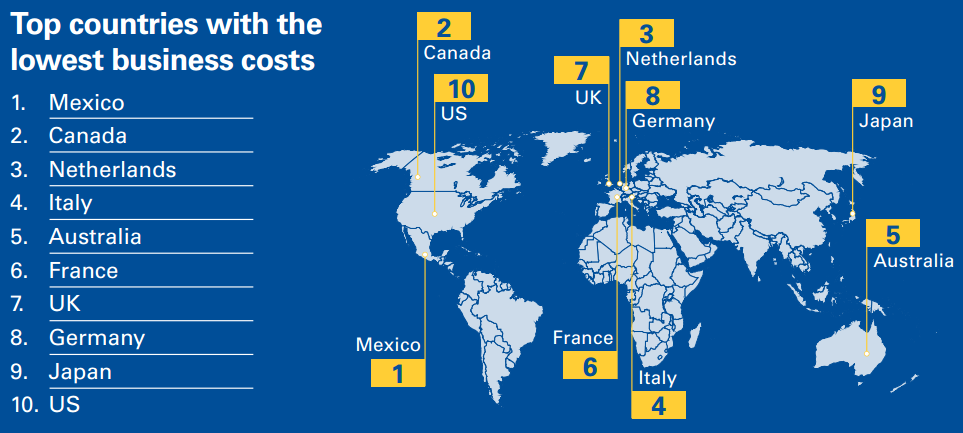
\includegraphics[width=11.5cm]{../pics/KPMG2016-top10-countries-wlow-bizcosts}
	\end{figure}
}

\frame{
	\frametitle{Global Competition}
	\framesubtitle{Business Cost Advantage: Greater Toronto vs USA (York Region, 2016)}
	\begin{figure}
	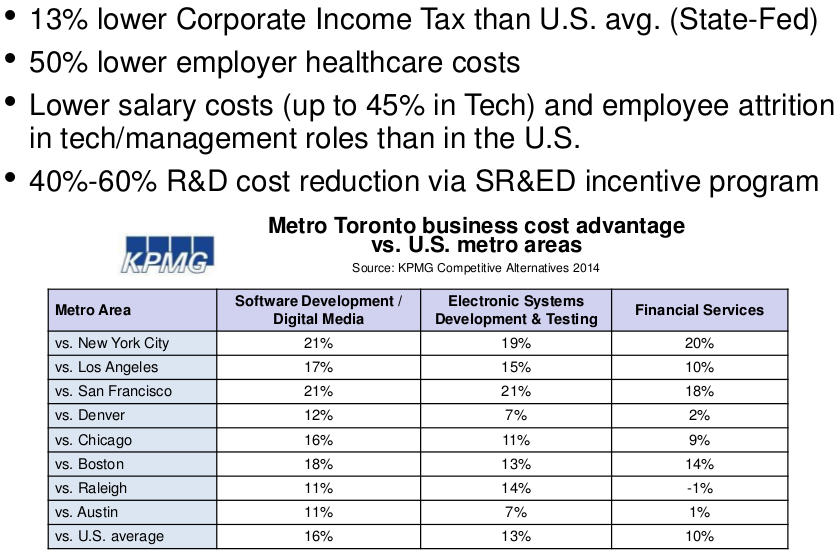
\includegraphics[height=7.5cm]{../pics/York-GTA-cost-advantage-vs-USA}
	\end{figure}
}

\frame{
	\frametitle{Global Competition}
	\framesubtitle{Manufacturing Competitiveness (Global Top 10 from \href{https://www2.deloitte.com/global/en/pages/manufacturing/articles/global-manufacturing-competitiveness-index.html}{\cite{deloitte2016}})}
	\begin{figure}
	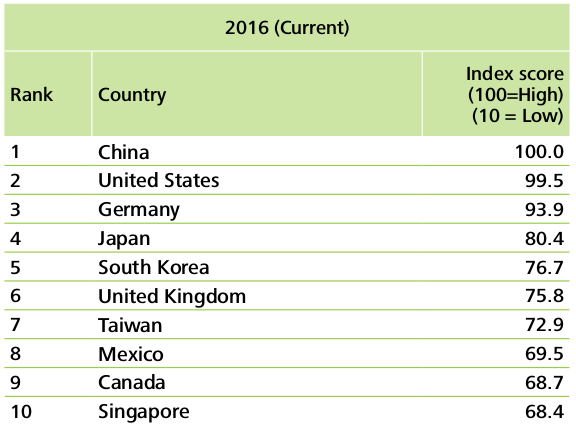
\includegraphics[height=7.5cm]{../pics/deloitte2016-top10-manufacturing-competitiveness}
	\end{figure}
}

\frame{
	\frametitle{Global Competition}
	\framesubtitle{Global Competitiveness Index (Global Top 15 from \href{http://www3.weforum.org/docs/gcr/2015-2016/Global_Competitiveness_Report_2015-2016.pdf}{\cite{wef}})}
	\begin{figure}
	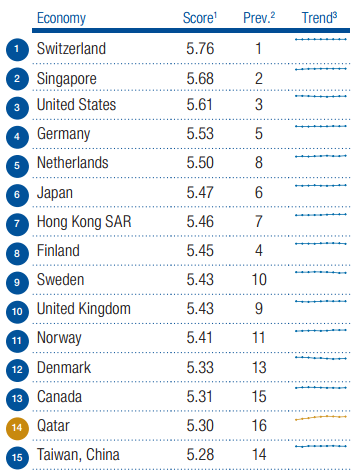
\includegraphics[height=7.5cm]{../pics/wef2016-global-competitiveness-index}
	\end{figure}
}

\frame{
	\frametitle{Global Competition}
	\framesubtitle{VC Money Invested in North American Cities (Thomson Reuters, 2016)} % First nine months of 2016 
	\begin{figure}
	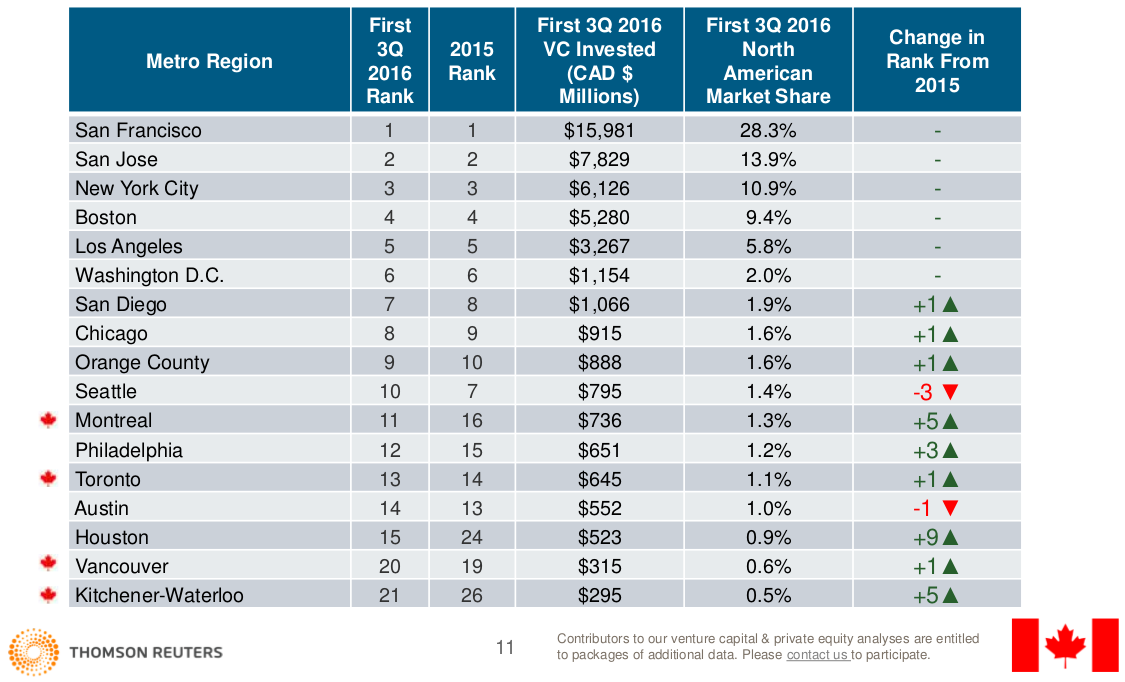
\includegraphics[height=7.4cm]{../pics/thomsonreuters2016-VC-funding-NA}
	\end{figure}
}

\frame{
	\frametitle{Global Competition}
	\framesubtitle{ICT Cluster Density across Canada (York Region, 2016)}
	\begin{figure}
	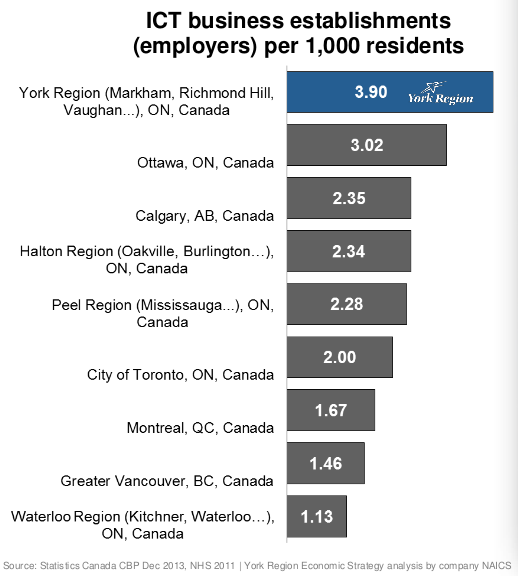
\includegraphics[height=7.5cm]{../pics/York-Canada-ICT-business-density}
	\end{figure}
}

\frame{
	\frametitle{Global Competition}
	\framesubtitle{Size of Ontario ICT Clusters (York Region, 2016)}
	\begin{figure}
	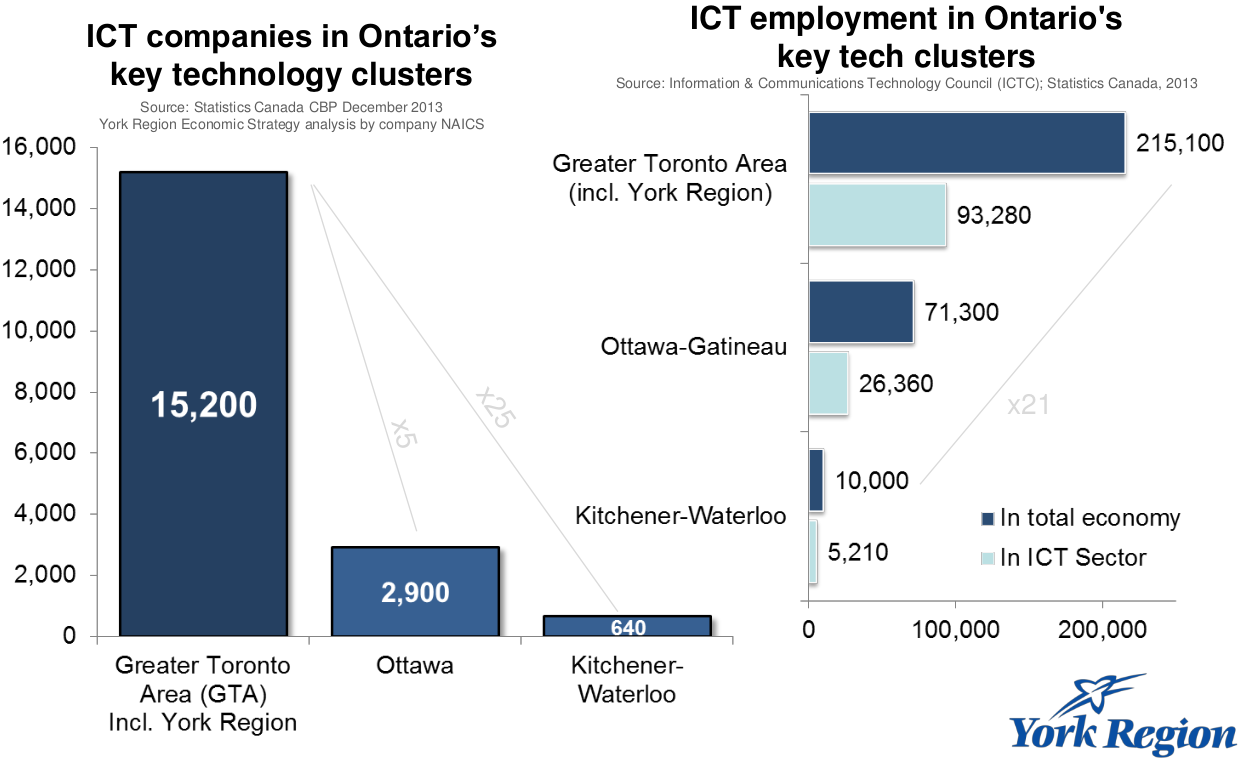
\includegraphics[height=7.4cm]{../pics/York-ICT-cluster-size}
	\end{figure}
}

\frame{
	\frametitle{Global Competition}
	\framesubtitle{Top Canadian Cities by Diversification (\href{https://techtoronto.org/Report2016/}{\cite{techto}})}
	\begin{figure}
	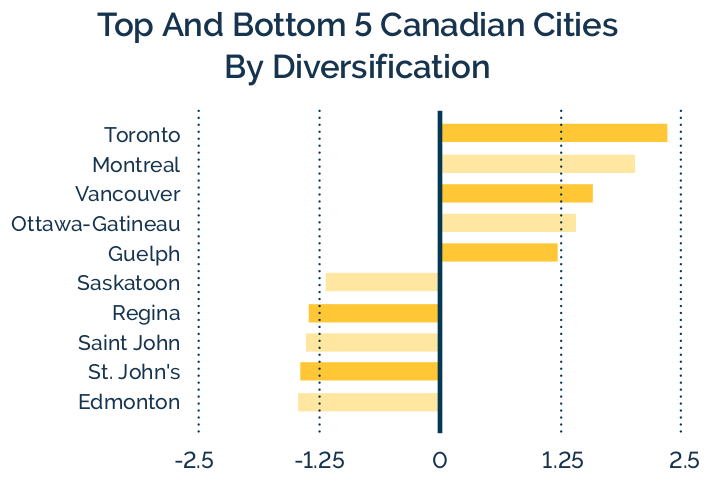
\includegraphics[height=6cm]{../pics/TechTO2016-Top-Canadian-Cities-by-Diversification}
	\end{figure}
}

\frame[allowframebreaks]{
	\frametitle{Global Competition -- References}
	%\framesubtitle{References}
	% keyword refers to bib file: references-KEYWORD.bib, and to the Tex file: section-KEYWORD.tex
	\printbibliography[keyword=global-competition]
}



\end{document}

